% Options for packages loaded elsewhere
\PassOptionsToPackage{unicode}{hyperref}
\PassOptionsToPackage{hyphens}{url}
\PassOptionsToPackage{dvipsnames,svgnames,x11names}{xcolor}
%
\documentclass[
  letterpaper,
  DIV=11,
  numbers=noendperiod]{scrartcl}
\usepackage{amsmath,amssymb}
\usepackage{lmodern}
\usepackage{iftex}
\ifPDFTeX
  \usepackage[T1]{fontenc}
  \usepackage[utf8]{inputenc}
  \usepackage{textcomp} % provide euro and other symbols
\else % if luatex or xetex
  \usepackage{unicode-math}
  \defaultfontfeatures{Scale=MatchLowercase}
  \defaultfontfeatures[\rmfamily]{Ligatures=TeX,Scale=1}
\fi
% Use upquote if available, for straight quotes in verbatim environments
\IfFileExists{upquote.sty}{\usepackage{upquote}}{}
\IfFileExists{microtype.sty}{% use microtype if available
  \usepackage[]{microtype}
  \UseMicrotypeSet[protrusion]{basicmath} % disable protrusion for tt fonts
}{}
\makeatletter
\@ifundefined{KOMAClassName}{% if non-KOMA class
  \IfFileExists{parskip.sty}{%
    \usepackage{parskip}
  }{% else
    \setlength{\parindent}{0pt}
    \setlength{\parskip}{6pt plus 2pt minus 1pt}}
}{% if KOMA class
  \KOMAoptions{parskip=half}}
\makeatother
\usepackage{xcolor}
\IfFileExists{xurl.sty}{\usepackage{xurl}}{} % add URL line breaks if available
\IfFileExists{bookmark.sty}{\usepackage{bookmark}}{\usepackage{hyperref}}
\hypersetup{
  pdftitle={Collaboration on the hub tooling},
  colorlinks=true,
  linkcolor={blue},
  filecolor={Maroon},
  citecolor={Blue},
  urlcolor={Blue},
  pdfcreator={LaTeX via pandoc}}
\urlstyle{same} % disable monospaced font for URLs
\usepackage{longtable,booktabs,array}
\usepackage{calc} % for calculating minipage widths
% Correct order of tables after \paragraph or \subparagraph
\usepackage{etoolbox}
\makeatletter
\patchcmd\longtable{\par}{\if@noskipsec\mbox{}\fi\par}{}{}
\makeatother
% Allow footnotes in longtable head/foot
\IfFileExists{footnotehyper.sty}{\usepackage{footnotehyper}}{\usepackage{footnote}}
\makesavenoteenv{longtable}
\usepackage{graphicx}
\makeatletter
\def\maxwidth{\ifdim\Gin@nat@width>\linewidth\linewidth\else\Gin@nat@width\fi}
\def\maxheight{\ifdim\Gin@nat@height>\textheight\textheight\else\Gin@nat@height\fi}
\makeatother
% Scale images if necessary, so that they will not overflow the page
% margins by default, and it is still possible to overwrite the defaults
% using explicit options in \includegraphics[width, height, ...]{}
\setkeys{Gin}{width=\maxwidth,height=\maxheight,keepaspectratio}
% Set default figure placement to htbp
\makeatletter
\def\fps@figure{htbp}
\makeatother
\setlength{\emergencystretch}{3em} % prevent overfull lines
\providecommand{\tightlist}{%
  \setlength{\itemsep}{0pt}\setlength{\parskip}{0pt}}
\setcounter{secnumdepth}{-\maxdimen} % remove section numbering
\KOMAoption{captions}{tableheading}
\makeatletter
\makeatother
\makeatletter
\@ifpackageloaded{caption}{}{\usepackage{caption}}
\AtBeginDocument{%
\renewcommand*\contentsname{Table of contents}
\renewcommand*\listfigurename{List of Figures}
\renewcommand*\listtablename{List of Tables}
\renewcommand*\figurename{Figure}
\renewcommand*\tablename{Table}
}
\@ifpackageloaded{float}{}{\usepackage{float}}
\floatstyle{ruled}
\@ifundefined{c@chapter}{\newfloat{codelisting}{h}{lop}}{\newfloat{codelisting}{h}{lop}[chapter]}
\floatname{codelisting}{Listing}
\newcommand*\listoflistings{\listof{codelisting}{List of Listings}}
\makeatother
\makeatletter
\@ifpackageloaded{caption}{}{\usepackage{caption}}
\@ifpackageloaded{subcaption}{}{\usepackage{subcaption}}
\makeatother
\makeatletter
\makeatother
\ifLuaTeX
  \usepackage{selnolig}  % disable illegal ligatures
\fi

\title{Collaboration on the hub tooling}
\author{}
\date{}

\begin{document}
\maketitle

\hypertarget{preface}{%
\subsection{Preface}\label{preface}}

The principles and guidelines presented in this document are inspired
from:

\begin{itemize}
\tightlist
\item
  communities / working groups in charge of defining widely used new
  standards, like the IETF and the W3C.
\item
  communities that have created and maintain universes of heavily
  interdependent packages, such as the
  \href{https://github.com/tidyverse}{tidyverse team}.
\item
  general good practice coding rules (e.g., semantic versioning).
\end{itemize}

\hypertarget{introduction-goals-and-expectations}{%
\subsection{Introduction: Goals and
expectations}\label{introduction-goals-and-expectations}}

\begin{figure}

{\centering 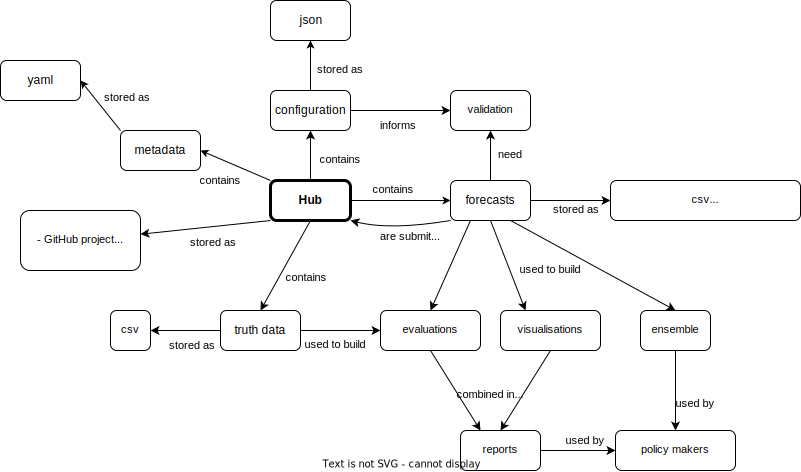
\includegraphics{concept_map.svg}

}

\caption{\label{fig-concept-map}\href{https://en.wikipedia.org/wiki/Concept_map}{Concept
map} of a modelling hub.}

\end{figure}

\begin{itemize}
\tightlist
\item
  Hub projects are complex, which present an challenge unusual for
  academics: developing while in production. Any breaking change in the
  infrastructure is made difficult by the fact that we don't break the
  workflow of our contributors.
\item
  Software development is complex. There is no foolproof method to
  design a perfect piece of software at the first attempt. Even the most
  talented and experienced software developers make changes they regret
  afterwards and are forced to create breaking changes.
\end{itemize}

Because of this double complexity, it is not likely that all teams will
converge towards using the same package at the same time. But this also
provides an opportunity: there is value in exploring independently
radically different technological solutions to a given problems. One of
the team might come across a solution that no other could have foreseen.

However, to keep a collaborative approach, where teams can adopt a
solution developed by others, and where we can all build on each other's
work, there are some technical pre-requisites:

\begin{itemize}
\tightlist
\item
  We need to agree on a common basis for all our future work: data
  format standards and shared design guidelines.
\item
  We need to build modular building blocks so transition to a different
  approach is easy and doesn't require changes throughout the ecosystem.
\end{itemize}

\hypertarget{data}{%
\subsection{Data}\label{data}}

As illustrated in Figure~\ref{fig-concept-map}, forecasts and the format
they use is one of the most central part of hubs. It therefore needs to
be the first point of discussion and agreement between hub teams.
Subsequent changes should be done via a versioning system to avoid
transmitting these breaking changes throughout hub tools.

\hypertarget{versioning}{%
\subsubsection{Versioning}\label{versioning}}

It is inevitable that data format will change over time as well. This is
a somewhat common situation when new formats develop and there are
plenty of examples to draw from to have a robust development process.
\href{https://www.w3.org/}{The W3C} is one of the champions of this
approach: SVG, HTML, CSS, WebExtensions, etc.\footnote{The IETF is
  another champion and delivered standards like the HTTP protocol.} In
this framework, every proposed modifications go through a heavily
codified selection process: First Public Working Draft, Revision of the
Working Draft, Candidate Recommendation, Proposed Recommendation,
Recommendation (illustrated in Figure~\ref{fig-w3c-process}, from
\href{https://www.w3.org/2021/Process-20211102/}{the W3C Process
Document}). You can see a live example by visiting the CSS Working Group
Current Work page: \url{https://www.w3.org/Style/CSS/current-work}.

\begin{figure}

{\centering \includegraphics{w3c_process.svg}

}

\caption{\label{fig-w3c-process}Detail of the W3C process to validate a
new standard.}

\end{figure}

This complex and somewhat rigid framework is necessary because of the
billions of users impacted by the recommendations. We might however want
a simpler system for the hub. Such a simpler model can be seen in the
json schema specification, where stable versions and draft
specifications coexist.

All hub teams should agree on a stable models and submit all proposed
changes for consideration to the other teams. If the proposed change
seem desirable, it should be added to the draft for the next version.

Each package can then specify with which version of the data format it
is compatible.

\hypertarget{individual-forecasts-vs-aggregated-forecasts-format}{%
\subsubsection{Individual forecasts vs aggregated forecasts
format}\label{individual-forecasts-vs-aggregated-forecasts-format}}

To reduce confusion and maintenance load, individual forecasts and
aggregated forecasts (e.g., as output by
\texttt{covidHubUtils::load\_forecasts()}) should have the same format.
Additional columns could potentially be added to aggregated forecasts
but the columns should always be a superset of the columns of individual
forecasts.

This allows tools to be used directly on individual forecasts, which may
be desirable for forecasters and hub maintainers in many situations.

\hypertarget{guidelines-for-universe}{%
\subsection{Guidelines for universe}\label{guidelines-for-universe}}

\hypertarget{modular-approach}{%
\subsubsection{Modular approach}\label{modular-approach}}

To ensure each team can easily swap individual pieces of their
infrastructure, it is important to ensure that the universe is modular.
Each package should focus on a single task (defined beforehand).

\hypertarget{avoiding-redundancy}{%
\subsubsection{Avoiding redundancy}\label{avoiding-redundancy}}

On a similar note, to avoid that changes in one piece of the
infrastructure ripple throughout the whole universe, overlap between
packages should be limited as much as possible.

The current hub infrastructure gives a good example of the maintenance
overhead due to overlap and redundancy across packages. As of 2021, the
submissions are checked for validated in the point during the pipeline:
during the submission process, when loaded with
\texttt{covidHubUtils::load\_forecasts()}, when uploaded to zoltar. This
means that any change in the data format requires changes in each one of
the 3 packages. Ultimately, it makes it more difficult to try to modify
\& improve the infrastructure.

\hypertarget{designing-general-tools}{%
\subsubsection{Designing general tools}\label{designing-general-tools}}

Since it can be difficult to predict how the other hubs will use the
packages your team designed, it is good practice to start with a very
streamlined architecture, with few features. It is easier to add
features \& complexity later down the line once other hubs agreed to the
proposed new features than to try and simplify an existing package.

If the tool can be made usable outside the context of hubs, it is even
better. Users are the most valuable and hardest to get feature of
research software. More users means more bugs uncovered, which is
crucial, since research software is often poorly tested.

\hypertarget{guidelines-for-individual-packages}{%
\subsection{Guidelines for individual
packages}\label{guidelines-for-individual-packages}}

\hypertarget{inputs}{%
\subsubsection{Inputs}\label{inputs}}

Whenever possible, the first input should be the data format defined in
\protect\hyperlink{data}{data}.

There should be tests ensuring that all functions return the same output
when fed with \texttt{data.frame}, \texttt{tibble} or
\texttt{data.table} since users might prefer to use one or the other in
the other steps of their workflow.

\hypertarget{outputs}{%
\subsubsection{Outputs}\label{outputs}}

Whenever possible, the output should be the data format defined in
\protect\hyperlink{data}{data}. Using the same format in input \& output
makes it easy for users to use functions in a pipeline with a previously
unanticipated order.

\hypertarget{lifecycle-versioning}{%
\subsubsection{Lifecycle \& versioning}\label{lifecycle-versioning}}

\hypertarget{semantic-versioning}{%
\paragraph{Semantic versioning}\label{semantic-versioning}}

It is likely that many packages from the universe will depend on others
packages from the universe, possibly maintained by another team. It is
therefore important to be able to identify breaking changes easily. The
most common pattern for this is to use
\href{https://semver.org/}{semantic versioning}, where breaking changes
are signified by the major version increase.

\hypertarget{sec-revdeps}{%
\paragraph{Reverse dependency checking}\label{sec-revdeps}}

Even with a modular structure, packages will be inevitably deeply
interconnected. This poses challenges regarding release timing. The
tidyverse for example already had to deal with complex issue on this
matter:

\begin{figure}

{\centering \includegraphics{images/paste-4C7C6C13.png}

}

\caption{Comment from Jenny Bryan on the reprex issue tracker: `The dev
version of reprex depends on the dev version of callr. So callr needs to
submit first. But the dev version of callr depends on the dev version of
processx. So processx needs to update first. And it has been stuck at
CRAN for months.'. Source:
\url{https://github.com/tidyverse/reprex/issues/171\#issuecomment-360996216}}

\end{figure}

To make sure updates are published in the correct order, all packages in
the universe should be set up for reverse dependency checking. This
service is provided for free by CRAN but since we did not decide yet if
all packages should be on CRAN, we should also set up our own reverse
dependency checking infrastructure.

\hypertarget{sec-advertising}{%
\paragraph{Update adversiting}\label{sec-advertising}}

Additionally, to make sure breaking changes are promptly addressed in
reverse dependencies, all new versions should be loudly announced to all
other teams. An issue way to do this would be to create a dedicated
slack channel with subscriptions to the relevant repository RSS feeds.

\hypertarget{release-cadence}{%
\paragraph{Release cadence}\label{release-cadence}}

??

See discussion at
\url{https://discuss.ropensci.org/t/release-cadence-how-do-developers-estimate-when-a-new-release-is-due/2861}

\hypertarget{questions-for-scope-assessment}{%
\subsection{Questions for scope
assessment}\label{questions-for-scope-assessment}}

\begin{itemize}
\tightlist
\item
  Could this package be accepted by CRAN in theory (even if you don't go
  through the actual submission process)?
\item
  Would this package work without any changes in someone started a hub
  in a new region (e.g., Africa or South America)?
\item
  To how many concepts or processes from Figure~\ref{fig-concept-map}
  does this package relate? The answer should probably be one in most
  cases.
\end{itemize}

\hypertarget{collaboration-communication}{%
\subsection{Collaboration \&
communication}\label{collaboration-communication}}

\hypertarget{centralized-organisation}{%
\subsubsection{Centralized
organisation}\label{centralized-organisation}}

To ensure constant quality across the universe and facilitate
infrastructure building (e.g. Section~\ref{sec-revdeps},
Section~\ref{sec-advertising}), it might make sense to group all
packages in a single GitHub organisation.

\hypertarget{governance}{%
\subsubsection{Governance}\label{governance}}

Complex projects with many moving parts and numerous collaborators need
a clear governance structure. If two collaborators disagree and cannot
resolve their disagreement through a discussion, what should be done? In
a typical academic article framework, the first author is usually
allowed to get the final say in these matters. But this system cannot
easily be transposed here.

First of all, in case of a disagree, there is nothing wrong with
agreeing to move in different directions for this specific piece of
infrastructure. As mentioned in the introduction of this document, there
is value in exploring different alternatives, as long as we make sure we
remain compatible.

However, this kind of split should remain limited because it takes off
time from an already very time-limited team. Open-source projects
usually deal with this situation by having a clear governance model in a
public document. A short and simple example of a governance model comes
from the tidyverse and ggplot2:
\url{https://github.com/tidyverse/ggplot2/blob/main/GOVERNANCE.md}.

\hypertarget{monthly-meetings}{%
\subsubsection{Monthly meetings}\label{monthly-meetings}}

To ensure communication stays active, we should book a slot for monthly
meetings. Additionally, to ensure equal footing of all teams or to
maintain engagement, a rotating schedule should be established. Each
team will be responsible for presentation one existing or planned piece
of infrastructure. This should facilitate exchange of workflow pieces
between teams and facilitate communication and identification of
possible incompatibility.

\end{document}
